\chapter{Test} \label{test} %<-- remember to label your test so you can
\textbf{Name: Group 630}\\  %    reference in the appropriate section
\textbf{Date: 21/02 - 2016}

\subsubsection{Purpose}
The purpose of the test.

\subsubsection{Setup}
\begin{figure}[H]
  \centering
	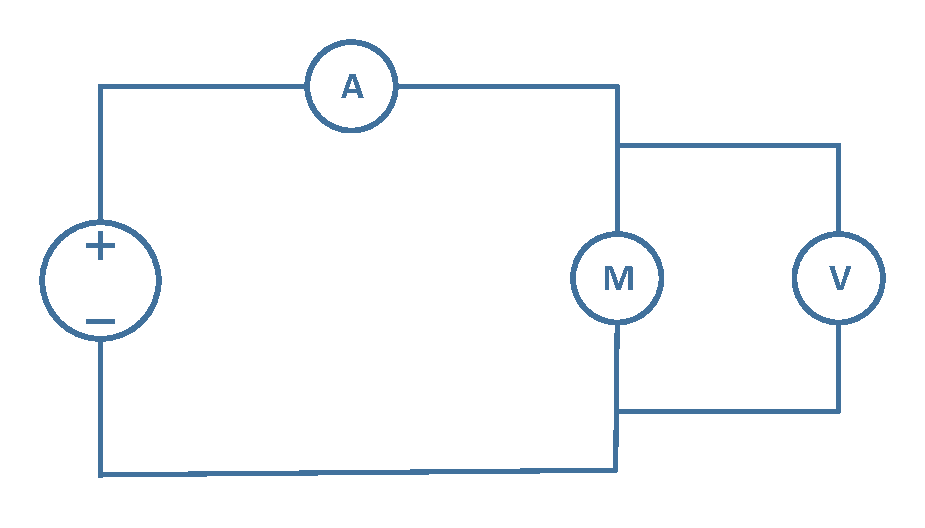
\includegraphics[scale=.45]{figures/MotorTest1.pdf}  %<-- These should be made in something
	\caption{Setup diagram}                              %    else than what this was made in
\end{figure}\vspace{-5mm}                              %    possibly CircuitTikZ for small
                                                       %    conceptual circuits like this.
\subsubsection{List of Equipment}
\begin{table}[H]
\begin{tabular}{|l|l|p{4cm}|}
\hline%------------------------------------------------------------------------------------
  \textbf{Instrument}                        &  \textbf{AAU-no.}  &  \textbf{Type}       \\
\hline%------------------------------------------------------------------------------------
  Multimeter 1                               &  60764             &  Fluke 189 True RMS  \\
\hline%------------------------------------------------------------------------------------
  Multimeter 2                   		         &  60769             &  Fluke 189 True RMS  \\
\hline%------------------------------------------------------------------------------------
  Power Supply \small{(0 - 32 V) (0 - 10 A)} &  77076             &  Ea - ps 7032 - 100  \\
\hline%------------------------------------------------------------------------------------
  Clamp for fixing the motor                 &  03039             &                      \\
\hline%------------------------------------------------------------------------------------
\end{tabular}
\end{table}

\subsubsection{Procedure}

\begin{enumerate}
  \item Turn on the two multimeters and choose Voltage and Ampere settings respectively.
  \item Fix the motor shaft so it can not turn.
  \item Choose the first current value (\SI{0,}{A}) on the current limiting of the power supply.
  \item Turn on the power supply and adjust the current limiting in accordance with the ampere meter.
  \item Read the voltage supplied to the motor from the volt meter.
  \item Repeat the three previous steps for each measurement in \SI{0,5}{A} increments up to 5 A.
  \item Switch the poles of the power supply and repeat the measurements in the negative direction.
\end{enumerate}

\subsubsection{Results}

\begin{table}[H]
\centering
\begin{tabular}{|l|l|l| l|l|}
\cline{1-2}\cline{4-5}%-----------------------             ----------------------------------------------
  \textbf{Input (A)}   & \textbf{Output (V)} &\phantom{hey}& \textbf{Input (A)}   & \textbf{Output (V)}\\
\cline{1-2}\cline{4-5}%-----------------------             ----------------------------------------------
  \SI{-5,0}{}          &       \SI{-0,71}{}  &             & \SI{0,5}{}           & \SI{0,16}{}        \\
\cline{1-2}\cline{4-5}%-----------------------             ----------------------------------------------
  \SI{-4,5}{}          &       \SI{-0,65}{}  &             & \SI{1,0}{}           & \SI{0,34}{}        \\
\cline{1-2}\cline{4-5}%-----------------------             ----------------------------------------------
  \SI{-4,0}{}          &       \SI{-0,59}{}  &             & \SI{1,5}{}           & \SI{0,53}{}        \\
\cline{1-2}\cline{4-5}%-----------------------             ----------------------------------------------
  \SI{-3,5}{}          &       \SI{-0,54}{}  &             & \SI{2,0}{}           & \SI{0,62}{}        \\
\cline{1-2}\cline{4-5}%-----------------------             ----------------------------------------------
  \SI{-3,0}{}          &       \SI{-0,43}{}  &             & \SI{2,5}{}           & \SI{0,64}{}        \\
\cline{1-2}\cline{4-5}%-----------------------             ----------------------------------------------
  \SI{-2,5}{}          &       \SI{-0,36}{}  &             & \SI{3,0}{}           & \SI{0,75}{}        \\
\cline{1-2}\cline{4-5}%-----------------------             ----------------------------------------------
  \SI{-2,0}{}          &       \SI{-0,27}{}  &             & \SI{3,5}{}           & \SI{0,78}{}        \\
\cline{1-2}\cline{4-5}%-----------------------             ----------------------------------------------
  \SI{-1,5}{}          &       \SI{-0,20}{}  &             & \SI{4,0}{}           & \SI{0,80}{}        \\
\cline{1-2}\cline{4-5}%-----------------------             ----------------------------------------------
  \SI{-1,0}{}          &       \SI{-0,14}{}  &             & \SI{4.5}{}           & \SI{0.83}{}        \\
\cline{1-2}\cline{4-5}%-----------------------             ----------------------------------------------
  \SI{-0,5}{}          &       \SI{-0,07}{}  &             & \SI{5.0}{}           & \SI{0.88}{}        \\
\cline{1-2}\cline{4-5}%-----------------------             ----------------------------------------------
\end{tabular}                                              %As you can see right above here, if you use
\end{table}                                                %\SI{}{} for numbers, it will replace '.' with ','
                                                           %because ',' is the SI standard.

\textbf{There are sometimes discussions about where to put the following. Sometimes it makes more sense to have it in the section where the test is used. Whichever way is chosen, should be consistent throughout the report.}

\begin{figure}[H]
  \centering
 	%Trim margins @:   left        bottom       right       top                 %  <--|If you feel like cropping a
 	\adjustbox{ trim = {.15\width} {.30\height} {.15\width} {.30\height}, clip }%  <--|pdf-file directly in latex :)
  {
    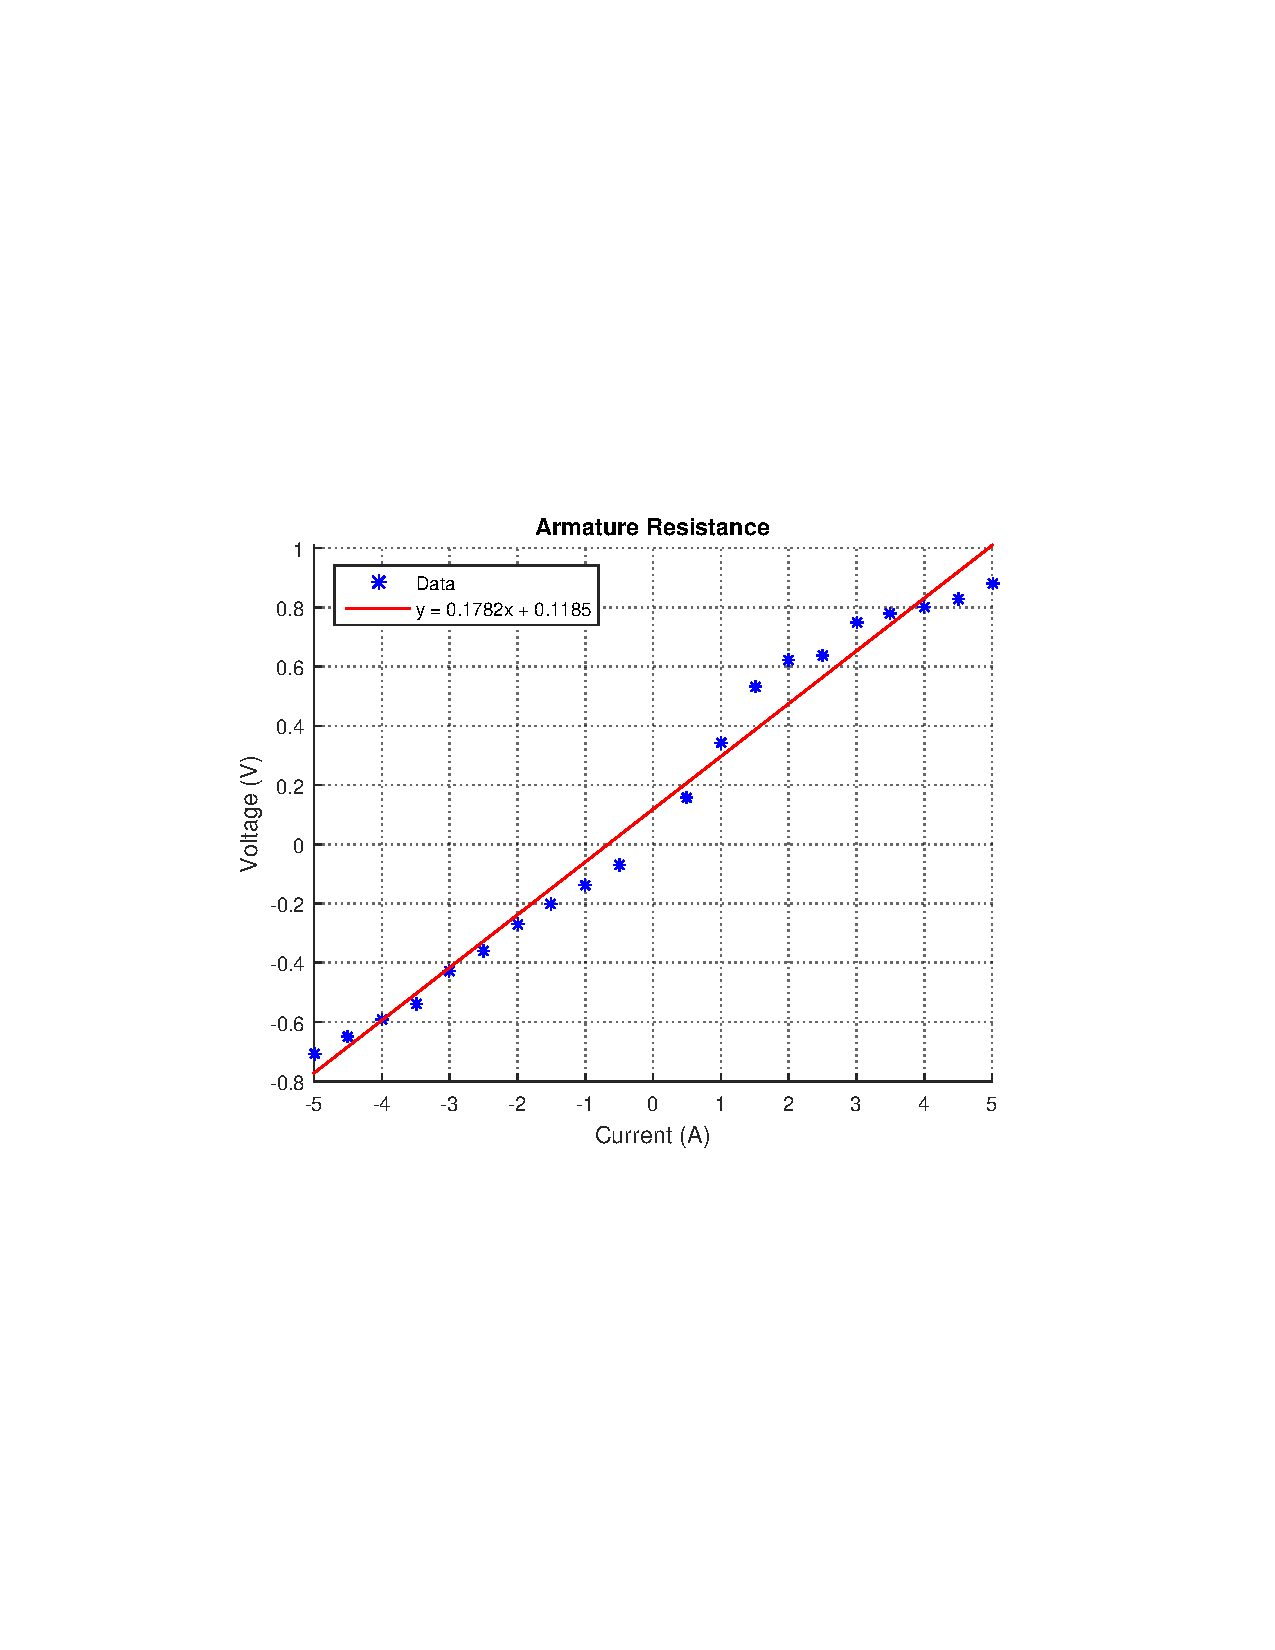
\includegraphics[width=\textwidth]{figures/armatureResistance.pdf}
  }
  \caption{A plot of a measured armature resistance, with a red line indicating the average value.}
  \label{armatureResistance}
\end{figure}

During these measurements the motor is in steady state. This is necessary for the inductor in the armature coil to act as a short circuit, which ease the calculation of the armature resistance. In steady state we get:

\begin{flalign}
  \eq{R_a} {\frac{U_a}{I_a}} \unit{\Omega}
\end{flalign}
\hspace{6mm} Where:\\
\begin{tabular}{p{1cm}lll}
  & \si{I_a} & is the armature current    &\unitWh{A}    \\
  & \si{U_a} & is the armature voltage    &\unitWh{V}    \\
  & \si{R_a} & is the armature resistance &\unitWh{\Omega}  \\
\end{tabular}

As seen on the data plot in \figref{armatureResistance} the result is a relatively linear function. The armature resistance is approximated directly as the slope of the least square line:
\begin{flalign}
  \eq{R_a}{\SI{0,178}{\Omega}}&
\end{flalign}